%  article.tex (Version 3.3, released 19 January 2008)
%  Article to demonstrate format for SPIE Proceedings
%  Special instructions are included in this file after the
%  symbol %>>>>
%  Numerous commands are commented out, but included to show how
%  to effect various options, e.g., to print page numbers, etc.
%  This LaTeX source file is composed for LaTeX2e.

%  The following commands have been added in the SPIE class 
%  file (spie.cls) and will not be understood in other classes:
%  \supit{}, \authorinfo{}, \skiplinehalf, \keywords{}
%  The bibliography style file is called spiebib.bst, 
%  which replaces the standard style unstr.bst.  

\documentclass[]{spie}  %>>> use for US letter paper
%%\documentclass[a4paper]{spie}  %>>> use this instead for A4 paper
%%\documentclass[nocompress]{spie}  %>>> to avoid compression of citations
%% \addtolength{\voffset}{9mm}   %>>> moves text field down
%% \renewcommand{\baselinestretch}{1.65}   %>>> 1.65 for double spacing, 1.25 for 1.5 spacing 
%  The following command loads a graphics package to include images 
%  in the document. It may be necessary to specify a DVI driver option,
%  e.g., [dvips], but that may be inappropriate for some LaTeX 
%  installations. 
\usepackage[]{graphicx}
\usepackage{epstopdf}
\usepackage{url}
\usepackage{amsmath}
\usepackage{enumerate}

\title{Unveiling ALMA software behavior using a decoupled log analysis framework}

%>>>> The author is responsible for formatting the 
%  author list and their institutions.  Use  \skiplinehalf 
%  to separate author list from addresses and between each address.
%  The correspondence between each author and his/her address
%  can be indicated with a superscript in italics, 
%  which is easily obtained with \supit{}.

\author{Juan Pablo Gil$\supit{a}^{*}$, 
Alexis Tejeda\supit{b}, 
Tzu-Chiang Shen\supit{a}, 
Norman S\'aez\supit{a}
\skiplinehalf
\supit{a}ALMA Joint Observatory\\
\supit{b}National Radio Astronomy Observatory\\ $*$jgil@alma.cl
%\supit{b}Affiliation2, Address, City, Country
}

%# atejeda : Atacama Large Millimeter/submillimeter Array, shouldn't be JAO ALMA Observatory ?

%>>>> Further information about the authors, other than their 
%  institution and addresses, should be included as a footnote, 
%  which is facilitated by the \authorinfo{} command.

\authorinfo{Further author information: Juan Pablo Gil: E-mail: jgil@alma.cl}
%%>>>> when using amstex, you need to use @@ instead of @
 

%%%%%%%%%%%%%%%%%%%%%%%%%%%%%%%%%%%%%%%%%%%%%%%%%%%%%%%%%%%%% 
%>>>> uncomment following for page numbers
% \pagestyle{plain}    
%>>>> uncomment following to start page numbering at 301 
%\setcounter{page}{301} 
 
  \begin{document} 
  \maketitle 

%%%%%%%%%%%%%%%%%%%%%%%%%%%%%%%%%%%%%%%%%%%%%%%%%%%%%%%%%%%%% 
\begin{abstract}
ALMA Software is a complex distributed system deployed roughly in more than one
hundred of computers, which interacts with more than one thousand of hardware
device components. A standard observation workflow interacts with the
distributed system, ALMASW, in a synchronized way. The Software Operation
Support team (SOFTOPS) comprises specialized software engineers, in which the 
team analyze dayly basis the generated log entries in order detect bugs, system 
failures and possibly predict eventual malfunctioning. 

A quick benchmark result, pointed that the log entries generated can reach, 
roughly, up to 30 GB per day and system instance running. It is proposed a 
decoupled and non-intrusive log analysis framework by using in-house developed 
tools and third-party library in order to identify well known problems, 
benchmaking, time profiling and
abnormal system behavior recongnition focused to alert the engineers to take 
corrective and preventive actions.

The key advantage of the proposed approach over other solutions is that the 
analysis itself does not interfere with the system resources in a production 
environment, allowing to execute concurrent log analyzer tools. 

In this paper, it is described the selected componentes of the framework, as 
well present the analized data.
\end{abstract}

%>>>> Include a list of keywords after the abstract 

\keywords{bug, detection, log, analyzer}

\renewcommand{\thefootnote}{\arabic{footnote}}

%%%%%%%%%%%%%%%%%%%%%%%%%%%%%%%%%%%%%%%%%%%%%%%%%%%%%%%%%%%%%
\section{INTRODUCTION}\label{sec:intro}  % \label{} allows reference to this section
The Atacama Large Millimeter/sub-millimeter Array (ALMA) is currently the
world's largest astronomical facility, built in partnership with Europe,
North America and East Asia in cooperation with the Republic of Chile. Its
frequency coverage has a range from the mm/submm windows up to 1 THz. The
observatory is placed in Atacama Desert at an altitude of 5000 meters above
sea level, and operates from the operations support facility at
2.900 meters.

The software that controls the overall operations of the array, data processing
and later storage is based on top of ALMA Common Software (ACS), which runs in
a highly distributed environment including hardware and computers. The logs
generated by the different components of software contains valuable information
such data rates, uncommon behaviour of hardware, times involved in the
different stages of observations, etc. However, due to the high amount of those
logs, most of that information remains hidden and are useless in practical terms,
except for a small set which is used to do daily troubleshooting activities.

A dedicated team of software engineers, SOFTOPS, provides frontline
software support for the ALMA software among other activities\cite{gonzalez2010first}.
The usual workflow is to receive problem reports and determine the root cause of
the failures. This task is done manually by analyzing the logs around the time of
the event and sometimes developing tools to extract specific information from
the whole set of logs in order to diagnose one specific problem. This approach
works well as a reactive measure to solve problems, but do not makes full usage
of most of the information contained the logs. As well, the time spent finding the
right logs among hundred or thousands of lines, can be in order of hours.

In this paper it is described generalities of ALMA software and its log system and
describe a on-going in-house development to make a better usage of the information
already being stored in the logs through automated tools that do not interfere
with the normal operation of an array.

\section{ALMA Software and Logging Service}
ALMA Common Software (ACS) is the framework used in the logical infrastructure
for ALMA operation. ACS is based on CORBA and provides low level services,
    network abstraction and common design patterns for distributed software,
    based in a component / container paradigm\cite{schwarz2004alma}.

%# atejeda : reference to the notification service
ACS by default, define a dedicated notify service\cite{notifyService} for the 
logging system that gets
distributed over the network based in a publish-subscribe paradigm used
intensively by ALMASW components. The logging service receives system-wide logs 
and distributes them to clients subscribed to the logging channel in a centralized
way. Each log has an associated priority and timestamp, allowing filtering at
different levels of the system. The logging channel consumers (clients) receives 
the log entries by subscribing to the event channel of interest.

A log entry is represented as a XML document composed by: 

{\small
\begin{verbatim}
<Debug 
  TimeStamp="2014-06-02T22:40:24.682" 
  File="acsServiceController.cpp" 
  Line="296" Routine="" 
  Host="10.197.52.10" 
  Process="acsservicesdaemon" 
  Thread="ACS Services Daemon Controller" 
  Context="" 
  SourceObject="ACS Services Daemon">
  <![CDATA[
    Imp 'Naming Service Imp' responded.
  ]]>
</Debug>
\end{verbatim}
}

\begin{itemize}
\item a timestamp encoded in ISO 8601 with precision up to millisecond
\item some fields of source code information like file, line and/or routine
\item runtime context information and origin, including host name, and thread
\item the priority of the log that covers from Trace (1) to Emergency (11)
\item the log message itself that is stored as CDATA\cite{avarias2010introducing}.
\end{itemize}

%# atejeda : meaning of jLog
In a standard ALMA production environment, a dedicated stack of computing 
hardware resources, is being used to operate ALMASW. 

% modified but this phrase doesn't make sense at all, which clients?
%There are, roughly,  of clients normally running during observation. 

The offical logging client used by the ALMA array operators is
jLog, a Java application that subscribes to the logging channel, receive the log 
entry and display it in a GUI with filtering and search capabilities. 
%% not used anymore : Another client redirects logs to a relational database, 
Concurrently, logs entries as a XML document, being archived in a FIFO scheme 
thirdparty service, typically, are kept up to two days due to hardware disk limitations.\cite{shen2012alma}.

\section{Decoupled Log Infrastructure}
Although the log information is available in XML documents, resides in the 
operation environment. Thus the data log analysis can not be performed using the 
same resources being used by the ALMASW, which, should be fully dedicated to 
operate the array, memory and CPU usage can not be shared for other non-critical 
ALMA operations. Due this, it was developed an in-house application that acts as 
a one way enterprise integration pattern routing and transportator, subscribed 
to the logging channel as a consumer and as a producer for thirdparty services, 
such as message queues and database.


% atejeda: to not saturate
The purpose of this architecture is to protect as much as possible the logging 
channel of ALMASW to not saturate the channel with non critical software operations, 
instead, by subscribing to a external message queue, RabbitMQ, deployed in a 
third-party service to gather or receive the log entries throughout this stack.

\begin{figure}[!ht]
 \begin{center}
 \begin{tabular}{c}
 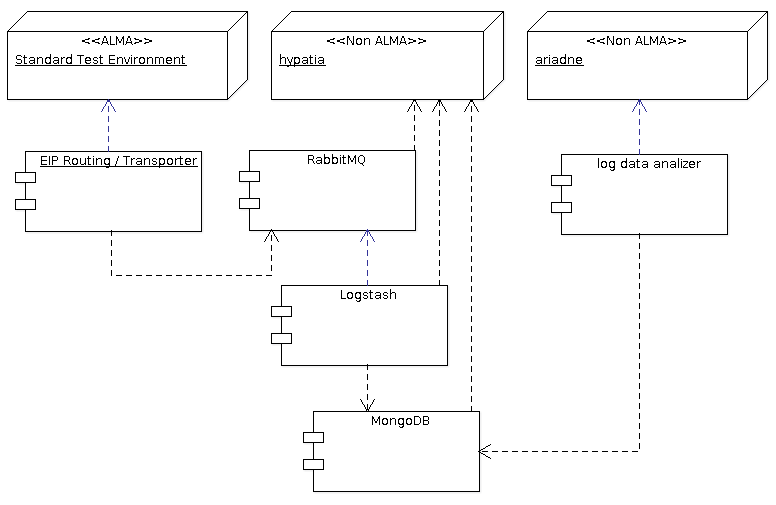
\includegraphics[height=9.0cm]{../img/DeploymentDiagram.png}
 \end{tabular}
 \end{center}
 \caption[dc] 
 { \label{fig:dc} Decoupled log architecture}
 \end{figure}

The infrastructure consists by a:

\begin{itemize}
\item Java client, subscribed to the logging channel, routing and transporting 
the messages to a message queue system
\item A queue message system, RabbitMQ\footnote{www.rabbitmq.com}, acting as a 
data log producer for the
\item A log manager, LogStash\footnote{www.logstash.com}, retrieves the data from 
the RabbitMQ, as a subscriber and archive it in a MongoDB instance.
\item A nosql database engine, MongoDB\footnote{www.mongodb.com}, with many collections 
as many ALMASW instances.
\end{itemize}

Currently, services are deployed in two environments, hypatia used for data 
management and ariadne, used for data analisys.

hypatia and ariadne specs.:

{\small
\begin{verbatim}
Linux 2.6.32-431.5.1.el6.x86_64
Intel(R) Xeon(R) CPU E5-2650 0 @ 2.00GHz
4 GB RAM x 4
120 GB DISK
\end{verbatim}
}

\section{Log Client}

The logging client, camel-acslog\footnote{https://github.com/atejeda/camel-acslog}, 
is a Apache Camel component \footnote{http://camel.apache.org/} and application 
which inherits the subscription managment classes of the jLog 
tool\footnote{ACS/ALMA Java GUI application} for the logging 
channel\cite{mora2012alma}. This client acts as a 
EIP\footnote{Enterprise Integration Pattern} by applying a message routing 
transalation, converting on the fly the XML entry to a Json 
data\footnote{fully compatible with the whole technology stack used} and adding 
to the Json data the origin of the log, STE hostname in order to be sent later 
to RabbitMQ.

{\small
\begin{verbatim}
{
  "_id" : ObjectId("5331d36c93f4348eef204d96"),
  "origin" : "system76",
  "uid" : "1387694615127_1",
  "date" : NumberLong("1387694615127"),
  "type" : "DEBUG",
  "file" : "SpectralProcessorTask.cpp",
  "line" : 1291,
  "routine" : "",
  "host" : "cob-cpn-09",
  "process" : "CORR/CDPNode/N09/cppContainer",
  "context" : "",
  "thread" : "SPT_3",
  "logMessage" : "[SPT_3] lags processing took: 3306 [us]",
  "sourceObject" : "SPT_3",
  "@timestamp" : "\"2013-12-21T23:43:35.127-07:00\""
}
\end{verbatim}
}

The camel-acs component, relies on a Java properties configuration, in which 
specify where the logs should be sent:

{\small
\begin{verbatim}
# allowed just one camel consumer endpoints
# use camel.endpoint.to.<unique_name> = <camel endpoint>
# camel.endpoint.from.acslog = acslog:?origin=${acslog.origin}
camel.endpoint.from = acslog:?origin=${acslog.origin}&xml=${acslog.xml}&mode=${acslog.mode}

camel.endpoint.to = \
  rabbitmq://${rabbitmq.broker}:${rabbitmq.port}/${rabbitmq.exchange}? \
  username=guest&password=guest&exchangeType=${rabbitmq.exchangetype}&routingKey=${rabbitmq.routing_key}
#camel.endpoint.to = stream:out
#camel.endpoint.to = mock:result
\end{verbatim}
}

The log client is a work still under 
development\footnote{http://mvnrepository.com/artifact/cl.alma.camel.acs/camel-acslog}, 
as ALMA is in production state, any addition and software changes must be carefully 
benchmarked and testedto certify that there is no critcal impact in a overall 
performance point of view. Preliminar tests results, showd that CPU usage and 
memory consumption is remains under control and 15 GB of data have been transferred 
to MongoDB without a critical impact in production environments.


\section{Message Queue and Database}
The log client consumer running within the environment production uses a instance 
of RabbitMQ as message broker, this message broker is configured as a topic 
exchange named as ALMA.

Logstash is in charge of mapping the log entry in order to be archived in a 
specific Mongo collection, this mapping is based on the origin field inserted at 
runtime, which represents the hostname where the log was produced by a ALMASW 
instance.\\

{\small
\begin{verbatim}
input {
    rabbitmq {
        host => "localhost"
        exchange => "ALMA"
        key => "alma.#"
        port => 15002
        codec => "json"
    }
}

output {
    mongodb {
        codec => "json"
        collection => "%{origin}"
        database => "almalogs"
        uri => "mongodb://localhost/almalogs"
    }
}
\end{verbatim}
}

It is important to notice:

1)  Origin: Besides production servers that controls the main array of antennas
(which is called ``AOS''), we have many small replicas with different
purposes like testing, commissioning, backup, etc. This field is used to
differentiate between sources, and also to store logs in separate collections
inside MongoDB. In RabbitMQ jargon\footnote{Advanced Message Queuing Protocol}, 
the field origin act as routing key.  

2) Date: ALMA Log message has a timestamp associated using the format
{\tt 2014-05-25T00:12:59.021 }. But searching strings over millions of logs
is inefficient, so we also store the number of milliseconds elapsed since Unix
Epoch (Jan 1, 1970).

For each origin there is a separate collection. Also, to control the size of
the database the collections are capped, that is, they acts as a FIFO queue if
the size of the database exceeds some limit. In our initial testing we
specified the max size parameter in 100 GB for AOS\footnote{ALMA Observatory Site, 
main enviroment used for science operations} and 10 GB for other
collections. For AOS it is expected to archive up to three days of normal operation
what is enough for the current analyzers that are already running.

The initial storage choice was ElasticSearch due it is straighforward
integration with LogStash. ElasticSearch is a is a indexer and realtime DSL searching framework, based on Apache Lucene\footnote{http://lucene.apache.org/core/}.

Even though, Elasticsearch is a powerfull and fast fremework to execute DSL queries
over several and huge amounts of data, there were three reasons to switch to MongoDB:

1) Even that the time response per query is the same, MongoDB has a deterministic and accurate search results, rather that the score systems that Elasticsearch offer which there is no guarantee of search accuracy for the same query in MongoDB.

2) there are other efforts inside ALMA that already uses MongoDB\cite{shenexploring}

The logs has a natural timing nature, and in order to use dates in an efficient
way MongoDB stores Date object using a 64 bit representation.

\section{Log Analyzers}
One common task of the software operation team is to diagnose the cause of errors
reported by array operators. Some the error are repeated, but in the
process to identify them as duplicated, hours can be spent. As a practical
application and to overcome that problem it was developed an error detector
script, given that the series of expected logs are known and can be identified uniquely. 

The purpose and approach is to search by queries to MongoDB, a predefined sequence of 
logs, acting like a simple pattern recongnition, if pattern match to a known error
pattern, then a specific error can be classified as detected.

A broad class of errors happens at some point inside one observation. An ALMA observation currently, from the functional point of view, has a very well defined and discrete workflow process, which consists in acquire observatory resources like antennas, 
perform the astronomical-phenomena observation, calibrate/reduce the
observed dataset and publish/archive the dataset. 

Every observation is executed within the context of one logical stackof hardware resources named as
Array. Can exists up to three concurrent arrays (TP\footnote{total power}, BL\footnote{baseline correlator}, ACA\footnote{ACA correlator}).


One of the problems faced is reduced the data log to detect a sequence of logs that could appears during an observation within the lifecycle of an array, up to three created arrays. The approach used was to represent the patter recognition by using FSM\footnote{Finite State Machine} due the simplicity, represented as a DFA\footnote{Deterministic Finite Automaton}, and flexibility for this specific problem. 

A sequence of logs that describes an error can be represented as a FSM if the EBNF\footnote{Extended Backus–Naur Form} grammar is well defined as the set of those logs, and the transition functions traversing different states describing the ordered steps of expected logs until the last one, ending in a ErrorDetected state. 

Due to the observation and array concepts described above, we also need to take
care about the lifecycles of the arrays and observations. So, any error
detector described by an FSM should include at least the array initialization
and array destructions states and his transitions. The observation as a lifecycle is an analogous work, so the approach will be focused only for the array lifecycle.

To implement the transition logic (or the specific logs that represent them), a script using Python and Pymongo library
was developed an implementation that creates a new FSM for each found array, search for each possible log given the current state, ordered by time, and considering only
the first element if any. If it exists, the FSM changes its state
accordingly and a new query is done until the last log is reached. If there
are no more logs, the script waits for more incoming logs and repeats the same transitions
until a final state is reached.

%-------------
   \begin{figure}[!ht]
   \begin{center}
   \begin{tabular}{c}
   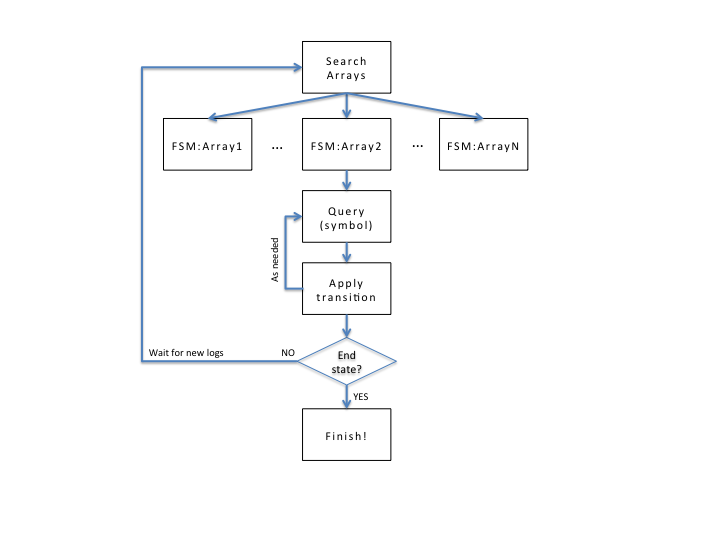
\includegraphics[height=8.0cm]{../img/FSM-flow-diagram.png}
   \end{tabular}
   \end{center}
   \caption[fsm] 
   { \label{fig:fsm} general state machine}
   \end{figure} 
%-------------

This script runs in Ariadne and querys Hypatia where MongoDB is deployed. The
program were done general: It reads the FSM specification from an external JSON
file. For example, the lifecycle array detector consists in this FSM
specification:
{\small 
\begin{verbatim}
{
  "StartState" : "InitArray",
  "FinalStates" : [ "CommitSuicide" ],
  "States": {
    "InitArray" : 
      [
        { 
          "query": {
              "logMessage": {"$regex": "successfully released a component with curl=this.arrayName$"},
              "sourceObject": "CONTROL/ACC/javaContainer"
              },
          "nextState" : "CommitSuicide"
        }
      ],
    "CommitSuicide" : []
  }
}

\end{verbatim}
}

And the output in a given set of logs (near 3 millions representing near 2 hours of real operation) is as follow:
{\small 
\begin{verbatim}
client-190-91-87-26:mongo joao$ ./testArray.py checkArrays.json
Using finite state machine: checkArrays.json
- New machine! CONTROL/Array001
- New machine! CONTROL/Array002
- New machine! CONTROL/Array003
--- CONTROL/Array001: "2014-03-21T20:31:32.534+00:00" client 'CONTROL/MASTER' has successfully 
released a component with curl=CONTROL/Array001
--- CONTROL/Array001: InitArray -> CommitSuicide
- Killing machine=CONTROL/Array001 because is in state CommitSuicide
- New machine! CONTROL/Array004
- New machine! CONTROL/Array005
--- CONTROL/Array002: "2014-03-21T20:40:33.051+00:00" client 'CONTROL/MASTER' has successfully 
released a component with curl=CONTROL/Array002
--- CONTROL/Array002: InitArray -> CommitSuicide
- Killing machine=CONTROL/Array002 because is in state CommitSuicide
- New machine! CONTROL/Array006
- New machine! CONTROL/Array007
--- CONTROL/Array004: "2014-03-21T20:50:30.522+00:00" client 'CONTROL/MASTER' has successfully 
released a component with curl=CONTROL/Array004
--- CONTROL/Array004: InitArray -> CommitSuicide
- Killing machine=CONTROL/Array004 because is in state CommitSuicide
--- CONTROL/Array006: "2014-03-21T21:39:46.518+00:00" client 'CONTROL/MASTER' has successfully 
released a component with curl=CONTROL/Array006
--- CONTROL/Array006: InitArray -> CommitSuicide
- Killing machine=CONTROL/Array006 because is in state CommitSuicide
It seems there is no more logs. Waiting 10 seconds until the new search.
It seems there is no more logs. Waiting 10 seconds until the new search.
It seems there is no more logs. Waiting 10 seconds until the new search.
Search disabled. Too much inactivity.
- Killing CONTROL/Array007 (InitArray) because I finished my searching and I will end.
- Killing CONTROL/Array005 (InitArray) because I finished my searching and I will end.
- Killing CONTROL/Array003 (InitArray) because I finished my searching and I will end.
\end{verbatim}
}

Extending this general behaviour is easy, but in order to see the real
performance of the system the log client that runs inside the production
servers must be installed and running continuously.

\section{Conclusions and Future Work}
It was presented in this work that heavy analysis can be done offline by using a
decoupled log database without interfere with normal and critical operation of the
observatory. This was done by deploying well known tools and some theoretical
concepts like FSM which can be extended to many other expected
behaviours or known errors. 

A number of direct improvements are possible in the infrastructure described
above. The logging client must be deeply tested so it became part of the
software, subject to formal maintenance by ALMA engineers. Many more FSM should
be deployed to effectively show the usefulness of the infrastructure in daily
support work. To help the scientist and operators, it could be developed GUIs
and web pages the display early alerts of failures. In the theoretical side,
the various finite state machines can be automatically merged in a bigger
one that reuses the input symbols shared between them (i.e. far less
queries to DB). 

As always, there are barriers for any new set of tools. Encouraging among team
members is necessary to exploit the full advantage of this system, at the price
of write one FSM for each desired sequence of events that it would be desirable
to monitor. The JSON format and direct queries in which the FSM is specified
should help to write checkers in few time so old known problems can be detected
automatically without spend hours trying to identify them or, even worse,
              happens unnoticed.

MongoDB has native implementations of LogReduce allowing to define complex
metrics and store them in separate collection to have historical analysis
without the need to keep the entire logs database for months or years. For
example, the development of a graphical interface that aggregates various
indicators of performance, so it would be easy to check at a glance if a new
software version is behaving at least as well as the previous one in terms of
performance and stability.
%\appendix    %>>>> this command starts appendixes
%%%%%%%%%%%%%%%%%%%%%%%%%%%%%%%%%%%%%%%%%%%%%%%%%%%%
%%%%%%%%%%%%%%%%%%%%%%%%%%%%%%%%%%%%%%%%%%%%%%%%%%%%%%%%%%%%%
%\acknowledgments     %>>>> equivalent to \section*{ACKNOWLEDGMENTS}       
 
%[...]

%%%%%%%%%%%%%%%%%%%%%%%%%%%%%%%%%%%%%%%%%%%%%%%%%%%%%%%%%%%%%
%%%%% References %%%%%

%\newpage
\acknowledgments{The Atacama Large Millimeter/submillimeter Array (ALMA), an
    international astronomy facility, is a partnership of Europe, North America
        and East Asia in cooperation with the Republic of Chile. ALMA is funded
        in Europe by the European Organization for Astronomical Research in the
        Southern Hemisphere (ESO), in North America by the U.S. National
        Science Foundation (NSF) in cooperation with the National Research
        Council of Canada (NRC) and the National Science Council of Taiwan
        (NSC) and in East Asia by the National Institutes of Natural Sciences
        (NINS) of Japan in cooperation with the Academia Sinica (AS) in Taiwan.
        ALMA construction and operations are led on behalf of Europe by ESO, on
        behalf of North America by the National Radio Astronomy Observatory
        (NRAO), which is managed by Associated Universities, Inc. (AUI) and on
        behalf of East Asia by the National Astronomical Observatory of Japan
        (NAOJ). The Joint ALMA Observatory (JAO) provides the unified
        leadership and management of the construction, commissioning and
        operation of ALMA.}
\bibliography{report}   %>>>> bibliography data in report.bib
\bibliographystyle{spiebib}   %>>>> makes bibtex use spiebib.bst

\end{document} 
